\section{Results}
\label{sec:results}

\subsection{Evidence coverage}
\label{sec:coverage}

\begin{table}[!t]
\caption{Attacker confirmation by evidence configuration, 30 seeds per cell.}
\label{tab:coverage}
\centering
\small
\begin{tabular}{@{}lccc@{}}
\toprule
Configuration & A1 & A2 & A3 \\
\midrule
Behavioural only & 3/30 & 30/30 & 30/30 \\
Localisation only & 30/30 & 0/30 & 30/30 \\
Fused & 30/30 & 30/30 & 30/30 \\
\bottomrule
\end{tabular}
\end{table}

\begin{figure}[!t]
\centering
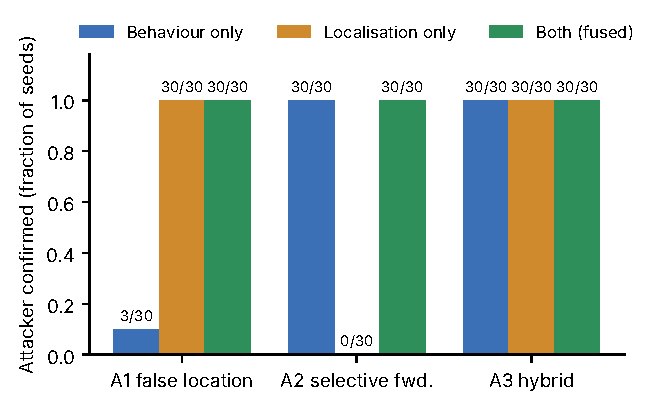
\includegraphics[width=0.78\textwidth]{fig2_coverage}
\caption{Evidence coverage over 30 seeds. Each single-evidence branch is
blind to the attack that produces no signature in its class; the three
behavioural confirmations of the A1 attacker occur at a lower rate than the
same branch confirms honest beacons.}
\label{fig:coverage}
\end{figure}

Table~\ref{tab:coverage} and Fig.~\ref{fig:coverage} report attacker
confirmation by evidence configuration. The inversion between the two
single-evidence rows admits a structural explanation. Under A1 the attacker
forwards honestly, so no behavioural quantity departs from its null
distribution. The delivered-throughput series of every A1 run is identical to
the clean-network run of the same seed, in all 30 seeds (Fig.~\ref{fig:tput}).
Behavioural evidence alone nevertheless confirmed the A1 attacker in 3 of 30
seeds. These confirmations carry no attack signal: on the clean network the
behavioural branch alone confirms honest beacons in 15 of 90 node-seeds (17\%),
a higher rate than its 10\% on the A1 attacker. Symmetrically, under A2 the
attacker advertises its true position, and localisation evidence alone
confirmed it in 0 of 30 seeds; it confirmed no honest beacon in any run of the
campaign.

A single-evidence detector therefore has a region of the attack space it
cannot observe, and an adversary who knows which evidence is collected may
choose to occupy it. This follows from what each evidence class can physically
observe, and no threshold setting changes it.

The scope of the claim is narrow. Table~\ref{tab:coverage} establishes that
collecting both classes covers both attacks. It does not establish that
Stouffer fusion is responsible: a disjunctive rule that thresholds each branch
independently and confirms on either would achieve the same result on A1 and
A2, because in each case one branch is far into its tail while the other is
silent. Fusion and disjunction separate only where both branches are weak
simultaneously. The coverage result is a result about evidence collection; the
fusion-rule question is taken up in Section~\ref{sec:sweep}.

\begin{figure}[!t]
\centering
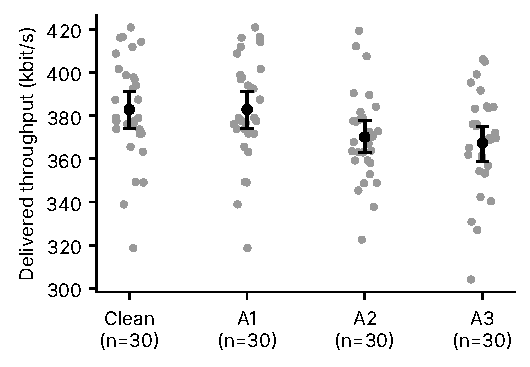
\includegraphics[width=0.6\textwidth]{fig3_throughput}
\caption{Delivered throughput by scenario, 30 seeds, with bootstrap 95\%
intervals of the mean. A1 and the clean network produce identical throughput
in every seed: the false-location attack has no packet-level footprint.}
\label{fig:tput}
\end{figure}

Two timing quantities are reported and must not be conflated. Detection
latency is the interval between attack onset and the first window in which the
attacker is confirmed. Isolation time is the timestamp of the first isolate
event written to the enforcement schedule. Over 30 seeds, the fused pipeline
confirmed the attacker in every seed of every attack. Median latency was
15.0\,s for A1 and A3 and 27.5\,s for A2 (means 20.0, 20.7 and 41.7\,s), with
a tail of slower confirmations reaching 80, 75 and 160\,s respectively.

The difference between attack classes is a property of the evidence, and the
model predicts its direction. Behavioural evidence reaches half confidence
weight at $n_{1/2} = 45$ observations against 5 for localisation
\eqref{eq:conf}. A2 is observable only through the behavioural branch, so its
confidence factor climbs an order of magnitude more slowly and confirmation
waits on the accumulation of transit packets. A1 and A3 are observable through
localisation, for which a handful of beacon receptions suffice. The constants were
fixed during calibration and not adjusted afterwards.

\subsection{Attack intensity and the fusion region}
\label{sec:region}

All three configurations confirm the A3 attacker in every seed, so the
experiment designed to show a fusion sensitivity advantage did not show one.
To locate where an advantage could appear we assume that branch anomaly
magnitude scales approximately linearly with attack intensity,
$A(f) \approx f A(1)$. For an RSSI-derived range residual under mobility, and
for a drop-rate statistic estimated from a finite window, that linearity is
plausible over a limited range but not guaranteed, so what follows locates the
region under an idealised model of the detector.

Let $\theta_B$ and $\theta_L$ be the intensities at which each branch alone
reaches the decision threshold, so that branch $X$ has anomaly
$\theta f/\theta_X$ at intensity $f$. With effective weights
$\tilde\omega_B, \tilde\omega_L$ the fused statistic of~\eqref{eq:stouffer}
crosses the threshold at
\begin{equation}
\label{eq:ffused}
f_F = \frac{\sqrt{\tilde\omega_B^{2} + \tilde\omega_L^{2}}}
           {\tilde\omega_B/\theta_B + \tilde\omega_L/\theta_L},
\end{equation}
and the family passes through a fusion-only region (an intensity at which
fusion confirms and neither branch does) precisely when
\begin{equation}
\label{eq:region}
f_F < \min(\theta_B, \theta_L).
\end{equation}
When the branches are equally sensitive the region is
$\theta_B/\sqrt2 < f < \theta_B$: a factor of $\sqrt2$ in intensity, half an
octave, and the widest it can be. Writing
$r = \max(\theta_B,\theta_L)/\min(\theta_B,\theta_L)$ for the sensitivity
ratio, \eqref{eq:region} with equal effective weights reduces to
\begin{equation}
\label{eq:ratio}
\frac{\sqrt{2}\,r}{1+r} < 1
\quad\Longleftrightarrow\quad
r < 1 + \sqrt{2} \approx 2.414 .
\end{equation}
With unequal weights, let $\tilde\omega_s$ weight the more sensitive branch and
$\tilde\omega_w$ the less sensitive one; the region exists if and only if
$r < \tilde\omega_w / \bigl(\sqrt{\tilde\omega_s^2 + \tilde\omega_w^2} -
\tilde\omega_s\bigr)$, which falls below $1+\sqrt{2}$ when the less sensitive
branch carries more weight (1.618 at twice the weight).

The condition concerns the attack family and not the detector, and the
distinction matters for how it is used. Write each branch's anomaly in units
of the decision threshold, $u = A_L/\theta$ and $v = A_B/\theta$, so that a
branch confirms alone when its coordinate reaches 1. With equal effective
weights the fused statistic confirms when $u + v \ge \sqrt2$, so the
fusion-only region is the triangle
\begin{equation}
\label{eq:wedge}
u < 1, \qquad v < 1, \qquad u + v > \sqrt2,
\end{equation}
which is non-empty for every equal-weight Stouffer detector, and with unequal
positive weights the corresponding region is non-empty as well. Every such
detector can therefore confirm attackers that neither branch confirms alone:
those whose two anomalies are each sub-threshold and of comparable normalised
size. Scaling an attack by intensity $f$ moves it along the ray
$(u, v) = f\,(1/\theta_L, 1/\theta_B)$ from the origin, and~\eqref{eq:ratio} is
the condition for that ray to pass through the triangle. A lopsided attack,
one that is much more visible to one branch than to the other, crosses the
more sensitive branch's threshold while the other branch's anomaly is still
too small to lift the fused statistic, and its ray misses the region. The ratio $r$ is therefore a property of how the
attack mixes the two misbehaviours, and it can be read from single-branch
detection curves for a given attack family before any fusion experiment is
run. Section~\ref{sec:sweep} tests it on two families that differ only in
that mix.

\subsection{False positives}
\label{sec:fp}

Over the 30-seed campaign the fused pipeline confirmed 9 of 90 honest
node-seeds on the clean network (10\%, Wilson 95\% interval 5.4--17.9\%) and 21
of 180 under attack (11.7\%, 7.8--17.2\%). The behavioural branch alone
confirmed 15 of 90 on the clean network and 35 of 180 under attack; the
localisation branch alone confirmed none. False confirmations are therefore a
property of the behavioural branch, whose peer-relative score fires whenever a
beacon's forwarding departs from its contemporaneous neighbours for benign
reasons such as mobility. Fusion with a silent localisation branch damps
these confirmations without removing them. With three monitored beacons per run, one false
positive moves per-run accuracy by 33 percentage points, which is why we
report counts instead of accuracy.

\subsection{Attack-intensity sweeps}
\label{sec:sweep}

We tested the fusion condition directly with two sweeps of the hybrid attack.
The primary sweep scales displacement and drop probability together from the
full-intensity A3 configuration over eleven levels, ten seeds each (110 runs,
Table~\ref{tab:sweep}). The second repeats eight levels with the drop
probability halved relative to displacement (80 runs, Table~\ref{tab:sweep2}).
Fig.~\ref{fig:sweep} shows both.

\begin{figure}[!t]
\centering
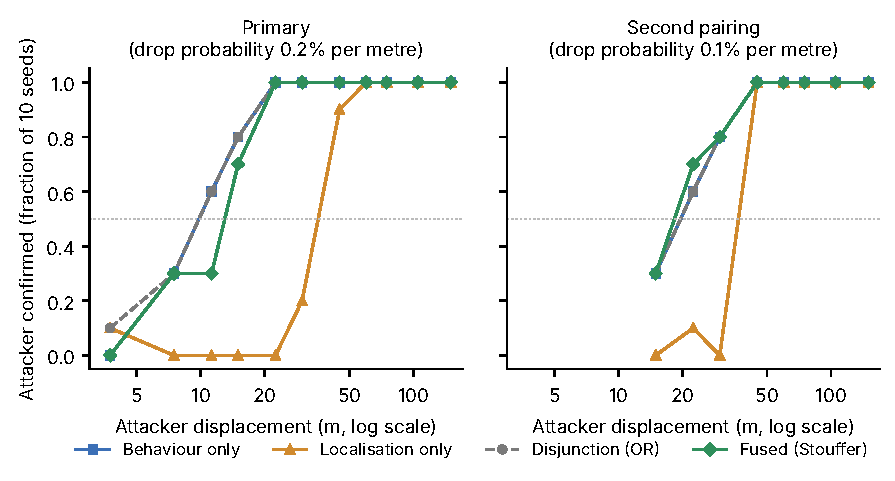
\includegraphics[width=\textwidth]{fig4_sweep}
\caption{Attacker detection across the two intensity sweeps, ten seeds per
point. Left: the branches' 50\% thresholds lie a factor of 3.63 apart, beyond the
$1+\sqrt2$ bound, and fusion falls below the disjunctive rule near the
behavioural threshold. Right: halving the drop rate moves the behavioural
curve and brings the ratio to 1.87, inside the bound, and fusion matches or
exceeds disjunction.}
\label{fig:sweep}
\end{figure}

\begin{table}[!t]
\caption{Primary sweep: attacker confirmed (of 10 seeds). Displacement is the
measured mean over the attacker's beacons after onset; below 45\,m it equals
the nominal $f\delta/2$ because the field boundary never clamps the offset.
Drop probability is $0.3f$. OR is the disjunctive rule over the
two single-evidence branches. FP counts honest beacons confirmed, of 20
node-seeds.}
\label{tab:sweep}
\centering
\small
\setlength{\tabcolsep}{4pt}
\begin{tabular}{@{}rrrrrrrr@{}}
\toprule
$f$ & Displ.\ (m) & Drop & Beh. & Loc. & OR & Fused & FP (OR / fused) \\
\midrule
0.025 & 3.75 & 0.0075 & 0 & 1 & 1 & 0 & 3 / 3 \\
0.05 & 7.5 & 0.015 & 3 & 0 & 3 & 3 & 5 / 4 \\
0.075 & 11.25 & 0.0225 & 6 & 0 & 6 & \textbf{3} & 1 / 1 \\
0.10 & 15.0 & 0.03 & 8 & 0 & 8 & \textbf{7} & 5 / 4 \\
0.15 & 22.5 & 0.045 & 10 & 0 & 10 & 10 & 5 / 5 \\
0.20 & 30.0 & 0.06 & 10 & 2 & 10 & 10 & 4 / 1 \\
0.30 & 45.0 & 0.09 & 10 & 9 & 10 & 10 & 4 / 4 \\
0.40 & 60.0 & 0.12 & 10 & 10 & 10 & 10 & 2 / 2 \\
0.50 & 74.9 & 0.15 & 10 & 10 & 10 & 10 & 3 / 2 \\
0.70 & 104.5 & 0.21 & 10 & 10 & 10 & 10 & 3 / 1 \\
1.00 & 147.1 & 0.30 & 10 & 10 & 10 & 10 & 3 / 3 \\
\bottomrule
\end{tabular}
\end{table}

\begin{table}[!t]
\caption{Second pairing: attacker confirmed (of 10 seeds) with drop probability
$0.15f$, half the rate of Table~\ref{tab:sweep}, at the same displacement.}
\label{tab:sweep2}
\centering
\small
\setlength{\tabcolsep}{4pt}
\begin{tabular}{@{}rrrrrrrr@{}}
\toprule
$f$ & Displ.\ (m) & Drop & Beh. & Loc. & OR & Fused & FP (OR / fused) \\
\midrule
0.10 & 15.0 & 0.015 & 3 & 0 & 3 & 3 & 5 / 4 \\
0.15 & 22.5 & 0.0225 & 6 & 1 & 6 & \textbf{7} & 1 / 1 \\
0.20 & 30.0 & 0.03 & 8 & 0 & 8 & 8 & 5 / 4 \\
0.30 & 45.0 & 0.045 & 10 & 10 & 10 & 10 & 5 / 5 \\
0.40 & 60.0 & 0.06 & 10 & 10 & 10 & 10 & 4 / 1 \\
0.50 & 74.9 & 0.075 & 10 & 10 & 10 & 10 & 2 / 2 \\
0.70 & 104.4 & 0.105 & 10 & 10 & 10 & 10 & 3 / 2 \\
1.00 & 147.1 & 0.15 & 10 & 10 & 10 & 10 & 3 / 2 \\
\bottomrule
\end{tabular}
\end{table}

\subsubsection{Primary sweep: the attack path misses the fusion-only region}

Behavioural detection falls from 8 of 10 at 15\,m to 6, 3 and 0 of 10 at 11.25,
7.5 and 3.75\,m; it reaches half detection at $\theta_B = 9.8$\,m, interpolated
on log intensity. Localisation evidence reaches half detection at
$\theta_L = 35.7$\,m. The measured ratio is $r = 3.63$. Resampling each level's
ten seeds as independent Bernoulli trials gives a bootstrap 95\% interval of
[2.67, 5.47], and fewer than 0.5\% of resamples fall below $1+\sqrt2$. Since
the less sensitive branch, localisation, carries the larger effective weight
through~\eqref{eq:conf}, the applicable bound is tighter still. This attack
family's path does not enter the fusion-only region.

The sweep shows the consequence the bound predicts. Where the behavioural
branch is near its threshold, adding the weaker localisation branch dilutes
it: at 11.25\,m fusion confirmed the attacker in 3 of 10 seeds against 6 for
the disjunctive rule, and at 15\,m in 7 against 8; at every stronger intensity
both confirmed it in all ten. The mechanism is visible at seed level. Where the
behavioural branch is anomalous and the localisation branch sits at its null,
equal-weight Stouffer combination computes $(A_B + 0)/\sqrt2$, attenuating a
live branch by 29\%, because a branch with adequate sample count carries
confidence weight whether or not it carries signal. Disjunction is immune,
since it never mixes the two. The same attenuation works in the opposite
direction for honest beacons: a benign behavioural deviation that would cross
the threshold alone is also scaled by $1/\sqrt2$ when the localisation branch
is at its null. Equal-weight fusion therefore trades sensitivity near the
threshold for suppression of single-branch false alarms. Sections~\ref{sec:fp},
\ref{sec:sparse} and~\ref{sec:scale} measure the second side of that trade.

\subsubsection{Second pairing: the condition predicts the outcome}

The ratio depends on how the sweep couples the two intensities, and the second
sweep tests whether~\eqref{eq:ratio} predicts the consequence. The behavioural
curve moved exactly as drop probability dictates: 3, 6 and 8 of 10 at drops of
1.5, 2.25 and 3\% in both sweeps, so behavioural detection depends on the drop
rate alone. Localisation, which depends on displacement alone, stayed close
to its primary-sweep value, at $\theta_L = 36.7$\,m. With $\theta_B = 19.7$\,m the ratio falls to $r = 1.87$
(bootstrap 95\% interval [1.41, 2.21]), inside the equal-weight bound in every
resample.

The outcome changed as the condition predicts. Fusion never confirmed fewer
attackers than the disjunctive rule. At $f = 0.15$, at which the behavioural
branch alone confirmed 6 of 10, fusion confirmed 7: one seed in which neither
branch crossed its threshold but their combined evidence did. One seed is weak
evidence and we do not report it as a fusion benefit. What the two sweeps
establish is that the same detector dilutes or helps depending on how the
attack family mixes its two misbehaviours, and that the ratio predicting which
can be measured before fusion is applied. The effective weights vary by window
through~\eqref{eq:conf}; if localisation carries twice the weight of behaviour,
the bound tightens to 1.618, which 17\% of resamples satisfy.

Taken together with Table~\ref{tab:coverage}, the finding is that evidence
collection determines coverage, and whether the combination rule adds anything
against a given attack family is decided by the branches' relative
sensitivity to that family.

\subsection{Comparison with literature baselines}
\label{sec:baselines}

Table~\ref{tab:baselines} compares the pipeline with the baselines of
Section~\ref{sec:baselinedef} on identical traces. The pipeline's false
isolation is that of policy E$'$, since the baselines also isolate on their
own detection and, like E$'$ in practice, do not release.

\begin{table}[!t]
\caption{Pipeline against literature baselines on identical traces. Detection
counts the attacker isolated after onset; FI is honest beacons isolated on the
clean network; $\bar\Phi$ is clean-network false isolation (E$'$ for the
pipeline); latency is the median time from onset to isolation, in seconds,
for A1 / A2 / A3, given only where the attacker was detected in at least half
the seeds. 30 seeds at 0\,dB and 20 under shadowing.}
\label{tab:baselines}
\centering
\small
\setlength{\tabcolsep}{3.5pt}
\begin{tabular}{@{}llcccccc@{}}
\toprule
$\sigma_{sh}$ & Method & A1 & A2 & A3 & FI & $\bar\Phi$ & Latency A1 / A2 / A3 \\
\midrule
0\,dB & LND & 30/30 & 2/30 & 30/30 & 3/90 & 0.003 & 10 / -- / 15 \\
      & WD & 1/30 & 30/30 & 30/30 & 4/90 & 0.031 & -- / 20 / 40 \\
      & LND+WD & 30/30 & 30/30 & 30/30 & 7/90 & 0.034 & 10 / 20 / 15 \\
      & Pipeline & 30/30 & 30/30 & 30/30 & 9/90 & 0.050 & 15 / 27.5 / 15 \\
4\,dB & LND & 20/20 & 1/20 & 20/20 & 2/60 & 0.005 & 15 / -- / 22.5 \\
      & WD & 4/20 & 20/20 & 13/20 & 7/60 & 0.050 & -- / 60 / 270 \\
      & LND+WD & 20/20 & 20/20 & 20/20 & 8/60 & 0.054 & 15 / 60 / 22.5 \\
      & Pipeline & 20/20 & 20/20 & 20/20 & 6/60 & 0.045 & 15 / 125 / 20 \\
8\,dB & LND & 20/20 & 0/20 & 20/20 & 1/60 & 0.000 & 20 / -- / 65 \\
      & WD & 0/20 & 20/20 & 3/20 & 0/60 & 0.000 & -- / 120 / -- \\
      & LND+WD & 20/20 & 20/20 & 20/20 & 1/60 & 0.000 & 20 / 120 / 65 \\
      & Pipeline & 20/20 & 20/20 & 19/20 & 0/60 & 0.000 & 22.5 / 150 / 155 \\
\bottomrule
\end{tabular}
\end{table}

The single-evidence baselines reproduce the coverage result with detectors
we did not design. The localisation-only detector revoked the A1 and A3
attackers in every seed of every channel and the A2 attacker in at most 2 of
30, and those few revocations came at least 225\,s after onset, at about the
rate at which it revoked honest beacons. The behaviour-only detector isolated
the A2 attacker in every seed and the A1 attacker in at most 4 of 20. Each
literature family is blind to the attack outside its evidence class, as
Table~\ref{tab:families} predicts from published descriptions.

The disjunction of the two baselines is the more instructive comparison, and
on it the pipeline does not win. LND+WD covered every attack in every channel
with false isolation statistically indistinguishable from the pipeline's: the
paired difference in clean-network $\Phi$ (pipeline minus LND+WD) was 19
node-seconds at 0\,dB (95\% CI $[-22, 61]$) and $-10$ at 4\,dB ($[-62, 43]$),
and both were zero at 8\,dB. It isolated attackers as fast or faster. The
pipeline was slower by a mean of 3.7\,s on A1 at 0\,dB (CI $[2.0, 5.2]$), by
60\,s on A2 at 4\,dB ($[18, 104]$) and by 77\,s on A3 at 8\,dB ($[33, 122]$),
and no paired interval showed it faster.

This is what Section~\ref{sec:region} predicts. A1 and A2 each disturb one
branch only, and A3 at its evaluated intensity lies above both branches'
individual thresholds rather than in the fusion-only region, so for every
attack evaluated here a disjunction loses nothing to fusion and
avoids the attenuation of a live branch by a silent one. The latency gap is
largest under shadowing, plausibly because the pipeline's behavioural branch
also waits for its confidence weight to saturate, which a reputation
threshold does not. In this network, therefore, the pipeline's detection is
matched by two calibrated classical detectors run in parallel.
Sections~\ref{sec:sparse} and~\ref{sec:scale} show that this does not carry
over to a sparse or a larger network; there the same disjunction withdrew
11--24\% of honest-beacon service against 0--3\% for the pipeline.

\subsection{Isolation policy under attack}
\label{sec:policy}

Table~\ref{tab:policy} and Fig.~\ref{fig:recovery} report the enforced runs of
the original campaign, five seeds per cell, and Fig.~\ref{fig:firstiso} the time
of first isolation under each policy over the 30-seed campaign. Detection is
identical across policies within each attack: the policies differ only in what
follows a verdict.

\begin{table}[!t]
\caption{Isolation policy comparison in the enforced runs, five seeds per cell.
Times in seconds, means over seeds; the attack begins at $t = 30$\,s. Policy C performs no
isolation.}
\label{tab:policy}
\centering
\small
\begin{tabular}{@{}llccc@{}}
\toprule
Attack & Policy & Isolation time & $R_{TH}$ & Recovery time \\
\midrule
A1 & C & -- & 0.97 & -- \\
   & D & 20.0 & 0.92 & 5.2 \\
   & E & 45.0 & 0.95 & 44.8 \\
A2 & C & -- & 0.93 & -- \\
   & D & 20.0 & 0.94 & 6.2 \\
   & E & 54.0 & 0.90 & 25.6 \\
A3 & C & -- & 0.93 & -- \\
   & D & 20.0 & 0.95 & 4.2 \\
   & E & 45.0 & 0.94 & 35.0 \\
\bottomrule
\end{tabular}
\end{table}

\begin{figure}[!t]
\centering
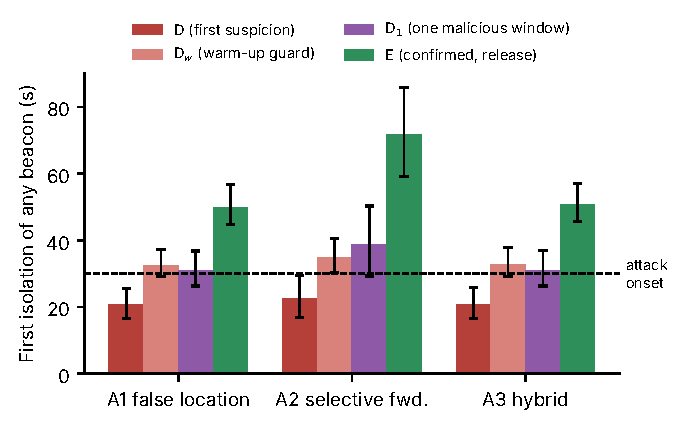
\includegraphics[width=0.78\textwidth]{fig5_first_isolation}
\caption{First isolation of any monitored beacon by policy, 30 seeds, with
bootstrap 95\% intervals. Policy D typically fires before the attack begins, so
what it first removes cannot be the attacker; D$_w$ and D$_1$ fire just after
onset, and E fires at onset plus detection latency.}
\label{fig:firstiso}
\end{figure}

Policy D first isolates at a median of 15\,s in every scenario, including the
clean network, before the attack begins at 30\,s. The 20.0\,s in
Table~\ref{tab:policy} is a five-seed mean (individual seeds 10--35\,s, median
20\,s), and is the same in all three attacks because the first isolation
precedes the attack and so depends only on the seed. The enforced runs used
the original campaign's calibration rather than the held-out seeds 101--105,
which moves one of the five seeds from 20 to 35\,s. What D removes at that point cannot be the
attacker. Its apparently fast recovery time of 4.2--6.2\,s is consequently an
artefact of having isolated before there was anything to recover from. D$_w$
and D$_1$ first isolate at medians of 30 and 35\,s. Policy E first isolates at
a median of 45\,s under A1 and A3 and 57.5\,s under A2, which is 30\,s plus the
corresponding detection latency: confirmation and enforcement coincide.

\begin{figure}[!t]
\centering
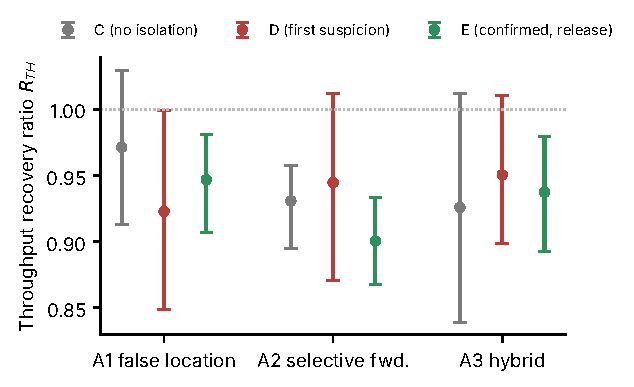
\includegraphics[width=0.68\textwidth]{fig6_recovery}
\caption{Throughput recovery ratio $R_{TH}$ in the enforced runs, five seeds,
with bootstrap 95\% intervals. The intervals exceed every between-policy
difference, so we claim no throughput advantage for any policy.}
\label{fig:recovery}
\end{figure}

Recovery ratios span 0.90--0.97 across all nine cells, with confidence intervals
substantially exceeding the differences between them (Fig.~\ref{fig:recovery}).
We claim no throughput advantage for any policy. Throughput debt, which we had
intended as a summary recovery metric, proved unusable: it returns non-zero
values on clean runs, because the baseline window is short relative to the
throughput variance of a mobile topology. Correcting it requires a later attack
start and a wider baseline window.

\subsection{Cumulative false isolation}
\label{sec:phi}

The comparison that separates the policies is not made under attack. On a clean
network every isolation is a false isolation, and $\Phi$ from~\eqref{eq:Phi} is
directly measurable. Table~\ref{tab:phivariants} and Fig.~\ref{fig:phi} report
it over 30 seeds for every policy, on the clean network and under each attack.

\begin{table}[!t]
\caption{Cumulative false isolation $\Phi$ (node-seconds) of honest beacons by
policy, 30 seeds. Honest isolated counts node-seeds; 95\% intervals are
percentile bootstrap over seeds. The final column is the paired difference from
policy E.}
\label{tab:phivariants}
\centering
\small
\setlength{\tabcolsep}{4pt}
\begin{tabular}{@{}llcrcc@{}}
\toprule
Network & Policy & Honest isolated & $\Phi$ & 95\% CI & $\Phi - \Phi_E$ [95\% CI] \\
\midrule
Clean & D     & 90/90 & 1052 & [1025, 1077] & 1005 [964, 1044] \\
      & D$_w$ & 90/90 & 1018 & [994, 1039]  & 971 [933, 1006] \\
      & D$_1$ & 88/90 & 897  & [843, 950]   & 851 [785, 911] \\
      & E     & 9/90  & 47   & [18, 79]     & -- \\
A1    & D$_1$ & 59/60 & 611  & [573, 648]   & 565 [519, 609] \\
      & E     & 8/60  & 47   & [18, 79]     & -- \\
A2    & D$_1$ & 58/60 & 587  & [532, 638]   & 557 [499, 612] \\
      & E     & 7/60  & 30   & [10, 54]     & -- \\
A3    & D$_1$ & 59/60 & 586  & [526, 639]   & 571 [514, 625] \\
      & E     & 6/60  & 15   & [2, 31]      & -- \\
\bottomrule
\end{tabular}
\end{table}

\begin{figure}[!t]
\centering
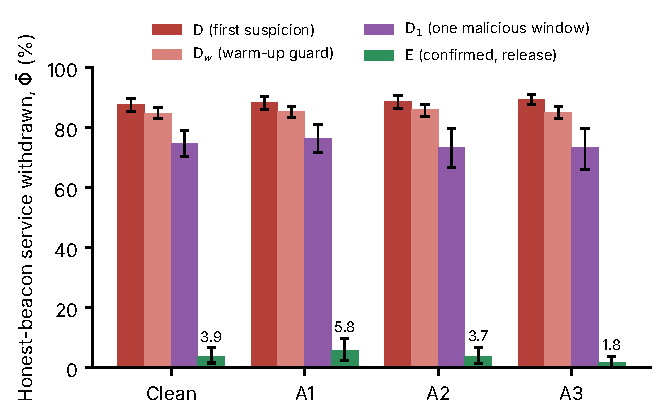
\includegraphics[width=0.8\textwidth]{fig8_phi}
\caption{Fraction of honest-beacon service withdrawn, $\bar\Phi$, by policy and
network, 30 seeds, with bootstrap 95\% intervals. Every immediate policy
withdraws 73--90\% of honest service; confirmation-gated isolation (E)
withdraws 2--6\%.}
\label{fig:phi}
\end{figure}

Policy D isolates on the first suspicious window, which typically falls before
any attacker is active. To test whether the comparison rests on a start-up
transient, D$_w$ ignores each beacon's first three usable windows, and D$_1$
isolates on the first window of malicious evidence without the persistence
requirement. On the clean network D$_w$ isolated all 90 honest node-seeds and
D$_1$ 88 of 90, with mean $\Phi$ of 1018 and 897 node-seconds against 47 for
policy E, which isolated 9 of 90. The paired difference between D$_1$ and E is
851 node-seconds (bootstrap 95\% CI [785, 911]); in normalised form D$_1$
withdraws 74.8\% of honest-beacon service and E 3.9\%. The advantage therefore
does not come from the start-up transient: removing the persistence requirement
alone is enough to isolate nearly every honest beacon. Under attack the same
ordering holds, and every paired interval excludes zero. Replaying the
original campaign's five clean seeds under that campaign's own calibration
gives D 1054 and E 49 node-seconds, inside the corresponding 30-seed
intervals. This checks the calibration and not the replay itself: both
figures are computed offline.

The replay itself was tested on clean seeds 1--10 by enforcing the replayed
schedules and rebuilding them from the verdicts issued under isolation
(Section~\ref{sec:method}). Isolation lowered $\Phi$ for both policies: D$_1$
from 910.5 to 829.5 node-seconds (paired difference $-81$, 95\% CI
$[-201.5, 45.5]$) and E from 32.5 to 24.5 (difference $-8$, CI $[-22, 0]$).
Neither interval excludes zero, and per seed the D$_1$ difference ranged from
$-370$ to $+295$, so the replay is unbiased within this resolution but noisy
for the immediate policy, and per-seed values of $\Phi$ for D$_1$ should not
be read individually. The comparison the paper rests on survived: under
isolation D$_1$ withdrew 69.1\% of honest-beacon service and E 2.0\%, D$_1$
exceeded E in all ten seeds, and the paired difference was 805 node-seconds
(CI $[693.5, 917]$) against 878 in the replay. For E the replay, if anything,
overstates $\Phi$.

The mechanism is that the policies inherit different bounds. Policy E isolates
only on confirmation, so its false-isolation rate is bounded by the detector's
false-confirmation rate of about 10\% (Section~\ref{sec:fp}). The immediate
policies isolate on weaker evidence, which on an uncontested network fires on
nearly every monitored beacon. The three-state verdict's contribution is the
tighter bound; it does not change what the detector can see.
Section~\ref{sec:release} shows that release contributes little to the gap.

The immediate policies are our own constructions, and the strongest of them,
D$_1$, isolates on a single window of evidence. Published schemes usually
wait for evidence to accumulate before they act: the localisation-only
baseline revokes a beacon only after more than $\tau'$ alerts, and the
behaviour-only baseline only after 20 packets of evidence. Both had low false
isolation in the dense network (0.3\% and 3.1\% of honest-beacon service,
Table~\ref{tab:baselines}). The comparison in Table~\ref{tab:phivariants} should
therefore be read as a measure of what acting before evidence accumulates
costs, not as a comparison with published practice. What the policies here
add is the size of that cost (about 75\% of honest-beacon service on a clean
network). Confirmation is one accumulation rule among several, and it was not
the cheapest in every network; Sections~\ref{sec:baselines},
\ref{sec:sparse} and~\ref{sec:scale} compare it with the two baselines.

\subsection{Release under isolation}
\label{sec:release}

The schedules above were built from verdicts issued while no beacon was
isolated. Re-verifying the enforced runs of the original campaign exposed a
behaviour that this construction hides. While a beacon is isolated it
forwards no transit traffic, so its behavioural branch falls below the
minimum sample: across the enforced runs behavioural evidence was usable in
1.6\% of the windows in which a beacon was isolated, against 54\% for the same
beacons and windows without isolation, while localisation evidence remained
usable in every window. For the A2 attacker, whose only signature is
behavioural, the fused trust therefore recovers once it is isolated. When the
E schedule was rebuilt from the verdicts issued under isolation, the A2
attacker was isolated at 45--65\,s and released at 115--160\,s in all five
seeds, after the twelve clean windows that clearing requires. A1 and A3
remained isolated, because their position lie keeps the localisation branch
in its tail. In a closed loop E would therefore cycle a forwarding attacker
between isolation and re-admission. Unlike timed redemption or an on--off
attack~\cite{bansal2003ocean,sun2006attacks}, this needs no timer and no
change in the attacker's behaviour. The replayed schedules contain milder
cases of the same effect: even without isolation, E released the attacker in
7 of the 90 attacked runs of the 30-seed campaign and in 3 of 60 at 4\,dB.

Policy E$'$ (Section~\ref{sec:framework}) releases a beacon confirmed on
behavioural evidence only when that evidence returns, which an isolated
beacon cannot supply. Its closed-loop schedule is therefore exact for those
beacons, which stay isolated, and follows the replay for beacons confirmed on
localisation alone. Table~\ref{tab:release} gives its cost.

\begin{table}[!t]
\caption{False isolation under evidence-aware release. $\bar\Phi$ is the
fraction of honest-beacon service withdrawn; E$'$ is evaluated as the closed
loop would run it. The last column is the paired difference D$_1 -$ E$'$ in
node-seconds with its bootstrap 95\% interval. 30 seeds at 0\,dB, 20 under
shadowing.}
\label{tab:release}
\centering
\small
\setlength{\tabcolsep}{4pt}
\begin{tabular}{@{}llcccc@{}}
\toprule
$\sigma_{sh}$ & Network & $\bar\Phi$ E & $\bar\Phi$ E$'$ & $\bar\Phi$ D$_1$ & D$_1 -$ E$'$ [95\% CI] \\
\midrule
0\,dB & Clean & 0.039 & 0.050 & 0.748 & 837 [773, 901] \\
      & A1    & 0.058 & 0.075 & 0.764 & 551 [500, 601] \\
      & A2    & 0.037 & 0.047 & 0.734 & 550 [486, 607] \\
      & A3    & 0.018 & 0.035 & 0.732 & 558 [497, 617] \\
4\,dB & Clean & 0.024 & 0.045 & 0.688 & 771 [677, 858] \\
      & A1    & 0.016 & 0.029 & 0.694 & 532 [475, 586] \\
      & A2    & 0.011 & 0.014 & 0.686 & 538 [482, 589] \\
      & A3    & 0.008 & 0.008 & 0.658 & 520 [445, 584] \\
8\,dB & Clean & 0.000 & 0.000 & 0.602 & 723 [656, 786] \\
      & A1    & 0.000 & 0.000 & 0.622 & 498 [452, 541] \\
      & A2    & 0.036 & 0.036 & 0.514 & 382 [321, 449] \\
      & A3    & 0.026 & 0.026 & 0.491 & 372 [298, 438] \\
\bottomrule
\end{tabular}
\end{table}

Evidence-aware release removed re-admission entirely: no attacker isolated
under E$'$ was released, in any of the 209 runs in which one was isolated. The
cost in false isolation was small. On the clean network $\bar\Phi$ rose from
3.9\% to 5.0\% (paired increase 13 node-seconds, 95\% CI [2, 28]), and E$'$
withdrew at most 7.5\% of honest-beacon service in any condition. The gap to
D$_1$ remained between 372 and 837 node-seconds, with every interval
excluding zero. The small cost has a simple cause: 46 of the 50 honest
beacons that E$'$ isolated across the three channels were never released, so
E$'$ amounts to near-permanent isolation on confirmation. Its advantage over
the immediate policies therefore comes from confirmation gating, not from
release. Release under E affected few honest beacons, and on the evidence
here a releasing policy is worth having only if it can distinguish recovered
evidence from absent evidence.

Iterating the loop confirmed both findings. Over three rounds on ten seeds,
E released the A2 attacker in every seed once its own enforced verdicts were
used: the fraction of post-onset time the attacker spent isolated fell from
0.88 in the first round to 0.23 in the second, and recovered only to 0.78 in
the third as the re-admitted attacker was confirmed again, the oscillation the
mechanism predicts. Under E$'$ the attacker was never released in any round
and spent 0.88 of the post-onset time isolated throughout. On the clean
network E$'$ was a fixed point from the first round in all ten seeds, with
$\Phi$ unchanged at 37 node-seconds, whereas E's $\Phi$ moved between rounds
(32.5, 24.5, 33.5) in two of the ten.

The A2 throughput and recovery rows of Table~\ref{tab:policy} were produced
by a schedule that never released the attacker. They are the rows E$'$ would
produce, not those of E in a closed loop.

\subsection{Robustness to shadowing}
\label{sec:shadow}

\begin{table}[!t]
\caption{Shadowing robustness, 20 seeds per cell. ``Confirmed'' is the fused
pipeline's attacker detections; latency is the median [interquartile range]
time from attack onset to confirmation, since the distributions are strongly
right-skewed; $\bar\Phi$ is the fraction of honest-beacon service withdrawn.
The $\sigma_{sh} = 0$ rows are the 30-seed campaign. In one 4\,dB seed the
beacon that later attacks was already falsely confirmed 5\,s before onset; in
the clean run of that seed the false confirmation cleared at 115\,s, but in
all three attack runs it persisted to the end, so the detection is counted.
Its latency is undefined and that seed is excluded from the latency columns.
It is also the single localisation confirmation of A2 at 4\,dB.}
\label{tab:shadow}
\centering
\small
\setlength{\tabcolsep}{4pt}
\begin{tabular}{@{}llccccc@{}}
\toprule
$\sigma_{sh}$ & Attack & Beh. & Loc. & Confirmed & Latency (s) & $\bar\Phi$ E / D$_1$ \\
\midrule
0\,dB & A1 & 3/30 & 30/30 & 30/30 & 15.0 [15.0--15.0] & 0.058 / 0.764 \\
      & A2 & 30/30 & 0/30 & 30/30 & 27.5 [15.0--52.5] & 0.037 / 0.734 \\
      & A3 & 30/30 & 30/30 & 30/30 & 15.0 [15.0--15.0] & 0.018 / 0.732 \\
      & Clean & -- & -- & -- & -- & 0.039 / 0.748 \\
4\,dB & A1 & 5/20 & 20/20 & 20/20 & 15.0 [15.0--15.0] & 0.016 / 0.694 \\
      & A2 & 20/20 & 1/20 & 20/20 & 125.0 [57.5--212.5] & 0.011 / 0.686 \\
      & A3 & 20/20 & 20/20 & 20/20 & 20.0 [15.0--32.5] & 0.008 / 0.658 \\
      & Clean & -- & -- & -- & -- & 0.024 / 0.688 \\
8\,dB & A1 & 0/20 & 20/20 & 20/20 & 22.5 [20.0--40.0] & 0.000 / 0.622 \\
      & A2 & 20/20 & 3/20 & 20/20 & 150.0 [101.2--215.0] & 0.036 / 0.514 \\
      & A3 & 14/20 & 18/20 & 19/20 & 155.0 [70.0--212.5] & 0.026 / 0.491 \\
      & Clean & -- & -- & -- & -- & 0.000 / 0.602 \\
\bottomrule
\end{tabular}
\end{table}

\begin{figure}[!t]
\centering
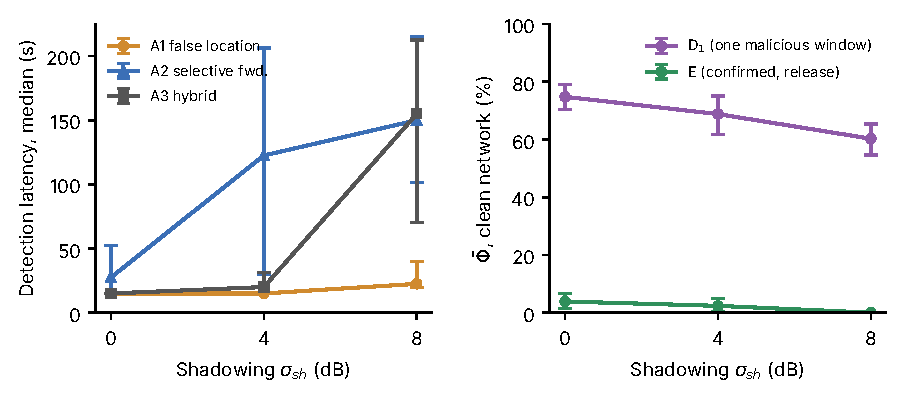
\includegraphics[width=\textwidth]{fig10_shadowing}
\caption{Effect of log-normal shadowing. Left: median detection latency, with interquartile range, rises sharply
for attacks seen through forwarding behaviour. Right: false isolation on the
clean network stays low for policy E and high for D$_1$.}
\label{fig:shadow}
\end{figure}

The campaign above uses a channel without shadowing, which flatters RSSI
ranging. We repeated it under log-normal shadowing with $\sigma_{sh} = 4$ and
8\,dB, 20 seeds per attack and channel. The pipeline was recalibrated on clean
runs of each channel, as a deployment would be; no threshold was changed.
Table~\ref{tab:shadow} and Fig.~\ref{fig:shadow} give the result.

Detection survived. The fused pipeline confirmed the attacker in every seed at
4\,dB and in 59 of 60 at 8\,dB, the miss being one A3 seed. The coverage
pattern held: localisation alone confirmed the A2 attacker in at most 3 of 20
seeds, and behaviour alone confirmed the A1 attacker in 5 of 20 at 4\,dB and
none at 8\,dB. Behavioural evidence degraded first: at 8\,dB it confirmed the
A3 attacker in 14 of 20 seeds, against 20 of 20 at 4\,dB. Shadowing adds link
loss that honest forwarders cannot control, which widens the peer distribution
the behavioural score is measured against.

The cost appeared as latency. Median time to confirmation for A2, the attack
visible only through forwarding, rose from 27.5\,s without shadowing to
125\,s at 4\,dB and 150\,s at 8\,dB; A3 rose to 155\,s at 8\,dB, once its
behavioural branch had degraded. A1, with its strong localisation signature,
was confirmed at a median of 15\,s at 4\,dB and 22.5\,s at 8\,dB.

False isolation did not grow. Policy E isolated at most 5 of 40 honest
node-seeds under attack and withdrew at most 3.6\% of honest-beacon service.
Recalibration widened the clean-network null enough that E isolated no honest
beacon in any clean 8\,dB seed. The immediate policies also isolated less as
the channel worsened, because the same widening raised their effective
threshold, but D$_1$ still withdrew 60--69\% of honest-beacon service on clean
networks, and the bootstrap intervals of D$_1$ and E did not overlap in any
condition.

\subsection{Sparse topology}
\label{sec:sparse}

Spreading the same 25 nodes over a $1000 \times 1000$\,m field changed the
balance of evidence. Behavioural evidence was usable in 18\% of windows,
against 52\% in the dense topology, while localisation evidence remained
usable in every window. Table~\ref{tab:sparse} gives the result.

\begin{table}[!t]
\caption{Sparse topology (25 nodes, $1000 \times 1000$\,m, 10 seeds).
Detection counts attackers isolated after onset (for the pipeline, confirmed);
latency is the median in seconds; FI and $\bar\Phi$ are for the clean network
(E$'$ for the pipeline). The single-branch rows count confirmations by each of
the pipeline's branches on its own. FI counts honest beacons isolated, except
for values marked $c$, which count honest beacons falsely confirmed by that
branch.}
\label{tab:sparse}
\centering
\small
\setlength{\tabcolsep}{4pt}
\begin{tabular}{@{}lccccc@{}}
\toprule
Method & A1 & A2 & A3 & FI & $\bar\Phi$ \\
\midrule
Pipeline & 10/10 & 4/10 & 10/10 & 0/30 & 0.000 \\
\quad latency & 62.5 & 132.5 & 62.5 & & \\
\quad behaviour branch only & 0/10 & 4/10 & 4/10 & 0/30$^{c}$ & -- \\
\quad localisation branch only & 10/10 & 0/10 & 10/10 & 0/30$^{c}$ & -- \\
LND & 10/10 & 0/10 & 10/10 & 0/30 & 0.000 \\
WD & 8/10 & 9/10 & 9/10 & 16/30 & 0.239 \\
LND+WD & 10/10 & 9/10 & 10/10 & 16/30 & 0.239 \\
Policy D$_1$ & & & & 8/30 & 0.100 \\
Policy D & & & & 30/30 & 0.849 \\
\bottomrule
\end{tabular}
\end{table}

The pipeline isolated no honest beacon in any sparse run, but it confirmed
the forwarding-only attacker in only 4 of 10 seeds and took a median of
62.5\,s to confirm the attacks with a localisation signature, four times the
dense figure. The cause is evidence scarcity: with few transit packets per
window the behavioural branch rarely reaches its minimum sample and its
confidence weight stays low. The behaviour-only reputation baseline, which
has no confidence weighting, isolated the A2 attacker in 9 of 10 seeds, but
on the clean network it also isolated 16 of 30 honest node-seeds and withdrew
23.9\% of honest-beacon service, because broken routes in a sparse network
look like dropped packets. The disjunction inherited both properties.

The single-branch rows locate the cause. The pipeline's own behavioural
branch, used alone, also confirmed no honest beacon, so fusion played no part
in the sparse result. What separates it from WD is how the behavioural
evidence is scored: against the beacon's neighbours in the same window, and
weighted by sample count. WD instead thresholds an absolute forwarding ratio.
The pipeline's behavioural branch therefore works as a peer-relative
behaviour-only detector, and in the sparse network it avoided the false isolation that the
absolute-ratio detector incurred, at the price of confirming the forwarding
attacker less often. The paired difference in clean-network $\Phi$ between the pipeline and LND+WD
was $-287$ node-seconds (95\% CI $[-446, -149]$), and the pipeline's $\Phi$
was lower under every attack as well (CIs excluding zero).

The comparison of Section~\ref{sec:baselines} therefore depends on the
topology. In the small dense network the disjunction matched the pipeline's
false isolation and was faster; in the sparse one it detected the forwarding
attacker more often but at roughly a quarter of honest-beacon service, which
is the trade $\Phi$ was introduced to expose. Section~\ref{sec:threats}
records a caveat on the sparse behavioural calibration.

\subsection{A larger network with two attackers}
\label{sec:scale}

Doubling the network to 50 nodes at the same density, with six monitored
beacons of which two attack simultaneously, left the main results in place
and sharpened the baseline comparison. Table~\ref{tab:scale} gives the
result.

\begin{table}[!t]
\caption{50-node network, two attackers, six monitored beacons, 10 seeds.
Detection counts runs in which both attackers were isolated after onset;
latency is the median over runs of the mean time to confirm the two
attackers, in seconds; FI and $\bar\Phi$ are for the clean network (E$'$ for
the pipeline). The single-branch rows count confirmations by each of the
pipeline's branches on its own. FI counts honest beacons isolated, except for
values marked $c$, which count honest beacons falsely confirmed by that
branch.}
\label{tab:scale}
\centering
\small
\setlength{\tabcolsep}{4pt}
\begin{tabular}{@{}lcccccc@{}}
\toprule
Method & A1 & A2 & A3 & Latency A1 / A2 / A3 & FI & $\bar\Phi$ \\
\midrule
Pipeline & 10/10 & 10/10 & 10/10 & 15 / 27.5 / 15 & 5/60 & 0.026 \\
\quad behaviour branch only & 0/10 & 10/10 & 10/10 & & 16/60$^{c}$ & -- \\
\quad localisation branch only & 10/10 & 0/10 & 10/10 & & 0/60$^{c}$ & -- \\
LND & 10/10 & 0/10 & 10/10 & 11.3 / -- / 17.5 & 2/60 & 0.005 \\
WD & 0/10 & 9/10 & 9/10 & -- / 20 / 67.5 & 7/60 & 0.108 \\
LND+WD & 9/10 & 9/10 & 9/10 & 12.5 / 20 / 15 & 9/60 & 0.113 \\
Policy D$_1$ & & & & & 60/60 & 0.742 \\
Policy D & & & & & 60/60 & 0.901 \\
\bottomrule
\end{tabular}
\end{table}

The pipeline confirmed both attackers in every attacked run, with medians of
15--27.5\,s, and isolated 5 of 60 honest node-seeds on the clean network.
Each single-evidence baseline was again blind outside its evidence class:
the localisation-only detector isolated no A2 attacker pair and the
behaviour-only detector no A1 pair. The coverage result therefore holds with
two simultaneous attackers and at twice the scale.

The disjunction of the baselines no longer matched the pipeline. It missed
one attacker in one run of each attack scenario, and its behavioural half
made it withdraw about four times as much honest-beacon service: 11.3\% on
the clean network against the pipeline's 2.6\%. Paired across
seeds, the pipeline's $\Phi$ was lower by 154 node-seconds under A2 (95\% CI
$[30, 277]$) and by 155 under A3 ($[42, 276]$); under A1 ($-163$,
$[-342, 8]$) and on the clean network ($-209$, $[-458, 0]$) the intervals
reached zero. Detection speed was indistinguishable: no paired latency
difference excluded zero. Immediate isolation was as costly as in the small
network, with D$_1$ withdrawing 72--74\% of honest-beacon service, and the
gap to E$'$ exceeded 1100 node-seconds under every scenario.

Here the cause is different from the sparse network. The pipeline's
behavioural branch alone falsely confirmed 16 of 60 honest node-seeds, more
than WD's 7, and the fused pipeline confirmed 5. The reduction from 16 to 5
is the attenuation of Section~\ref{sec:sweep} acting on honest beacons: a
benign behavioural deviation is scaled down by a localisation branch at its
null. Both counts come from the same topology and the same six-observer
median, so the observer count cannot explain the difference. At 50 nodes the
pipeline's lower $\Phi$ is therefore a benefit of fusion, and the dense
network shows the same effect on a smaller scale (15 of 90 honest node-seeds
for the behavioural branch alone against 9 fused).

Taken with Section~\ref{sec:sparse}, this bounds the baseline comparison of
Section~\ref{sec:baselines}. Only in the small dense network did two
classical detectors run side by side match the fused pipeline. In the sparse
network the advantage came from peer-relative scoring of behaviour, and at 50
nodes from fusion suppressing single-branch false alarms.

